%!TEX root = Thesis.tex

\chapter{Introduction}
The study of opinion is a one of the oldest fields, with roots in philosophy, going back to the Ancient Greek philosophers. The wide adoption of the Internet has made it possible for individuals to express their subjective opinions to an extent much more far-reaching then possible before. This has recently been intensified even more due to the explosive popularity of social networks and microblogging services. 

The amount of opinion data available is often huge compared to what traditional opinion analyses, e.g.\ questionnaire surveys, requires to yield significant results. Furthermore the opinions cover nearly every thinkable topic. This gives incentive, given that the potential value of such opinions can be great, if information can be extracted effectively and precisely. Given enough opinions on some topic of interest, they can yield significant indication of \emph{collective opinion shifts}, e.g.\ shifts in market trends, political sympathies, etc. 
%Feedback, in form of product and service reviews, can thus be highly valuable information for companies. Also political opinions are of high value for both governments and their the oppositions. 
The interest in such shifts is far from recent, and is a well established subfield of the \emph{psychometrics} and has strong scientific grounds in both psychology and statistics. 

However, since these opinions are often stated in an informal setting using natural language, usual methods developed for traditional opinion analyses, e.g.\ questionnaire surveys, cannot be directly applied on the data. The burst of computational power available has meanwhile made it possible to automatically analyze and classify these huge amounts of opinion data. The application of computational methods to extract such opinions are more commonly known as \emph{sentiment analysis}.

This thesis presents a \emph{formal logical method} to extract the \emph{sentiment} of natural language text reviews. In this chapter traditional methods for data collection of sentiments are briefly considered and thereafter the overall challenges involved in collecting reviews stated in natural language are presented. The opinions considered in this thesis are in form of product and service reviews, however most of the techniques presented can be generalized to other types of topics.

\section{Classical data collection}
One of the most used approaches to collect data for opinion analyses is through questionnaire surveys. Most of us are familiar with such surveys, where the subject is forced to answer questions with a fixed scale. For instance, given the statement ``The rooms at the Swissôtel Hotel are of high quality.'', a subject must answer by selecting one of a predefined set of answers, e.g.\ as shown in Figure~\ref{fig:LikertScale}.
\begin{figure}[ht]
	\begin{cframed}{.7\textwidth}
		\begin{enumerate}
		  \item Strongly disagree
		  \item Disagree
		  \item Neither agree nor disagree
		  \item Agree
		  \item Strongly agree
		\end{enumerate}
	\end{cframed}
	\caption{Likert scale.}
	\label{fig:LikertScale}
\end{figure}

Such scales, where the subject indicates the \emph{level of agreement}, are know as \emph{Likert scales}, originally presented by \citeauthor{Likert} \shortcite{Likert}, and has been one of the favorite methods of collection data for opinion analyses. Other scales are also widely used, for instance the \emph{Guttman scale} \cite{guttman}, where the questions are  binary (yes/no) and ordered such that answering yes to a questions implies the answer yes to all questions ordered below this. An example is shown in Figure~\ref{fig:GuttmanScale}. Thus the answer on both a Likert and a Guttman scale can be captured by a single \emph{opinion value}.
\begin{figure}[ht]
	\begin{cframed}{.7\textwidth}
		\begin{enumerate}
		  \item I like eating out
		  \item I like going to restaurants
		  \item I like going to themed restaurants
		  \item I like going to Chinese restaurants
		  \item I like going to Beijing-style Chinese restaurants
		\end{enumerate}
	\end{cframed}
	\caption{Guttman scale.}
	\label{fig:GuttmanScale}
\end{figure}

Given a set of answers, the result of such surveys are fairly easy to compute. At its simplest it can be a per question average of the opinion values, however it is mostly also interesting to connect the questions -- for instance how does subjects' answer to the above statement influent their answer to the statement ``The food at the Swissôtel Restaurant is of high quality.'', etc. 

One advantage of using fixed frameworks as the Likert and Guttman scales is that the result of the data collection is highly well-structured, and multiple answers are known to be provided by the same subject. This makes further analysis as the example just mentioned possible, something that will be much harder to achieve when harvesting reviews from the Internet, where the author of the review is presumably unknown, or at least not connected to any other reviews. Furthermore, since most questionnaire surveys are conducted in relatively controlled settings, where the subjects in many cases have been preselected to constitute a representative sample of some population, the results intuitively have relative high certainty.

However these properties also contributes to some of the disadvantages of classical data collection, namely the difficulty of getting people to answer them. Another issue is that people only can answer on the questions that are provided, which mean that significant aspects of the subjects opinion might not be uncovered if it is not captured by a question.

\section{Natural language data collection}
\label{sec:naturalDataCollection}

In this thesis it is argued that a far more natural way for subjects to express their opinions is through their most natural communication form, i.e.\ their language. The strongest incentive for considering natural language texts as a data source is simply the amount of data available through the Internet. This especially includes posts on social networking and microblogging services, e.g.\ \emph{Facebook}\footnote{Facebook, \url{http://www.facebook.com/}} and \emph{Twitter}\footnote{Twitter, \url{http://www.twitter.com/}}, where people often express the opinion on products and services, but also online resellers allowing their consumers to publicly review their producs such as \emph{Amazon}\footnote{Amazon, \url{http://www.amazon.com/}} 

%Clearly the first step needed is to harvest posts that actually concerns the topic of interest. 
This though introduces the need for efficient candidate filtering as the posts in general, of cause, are not constrained to a specific entity or topic of interest. This can be fairly easy achieved as most of the services provides APIs that allows keyword filtering.
%However it also significantly increases the data quantity, which in turn can yield a more precise analysis. 
The approach also raises ethical issues, since the author of the post might never realize that it is being used for the purpose of opinion analysis. Larger texts, such as blog posts, could indeed also be considered, however the contextual aspects of large, contiguous texts often makes interpretation extremely complex, thus making it a difficult task to extract opinions on a specific entity. In this thesis only relatively short reviews are thus considered.

One concern is whether texts harvested from the Internet can constitute a representative sample of the population in question. The actual population, of course, rely on the target of the analysis. This is a non-trivial study itself, but just to demonstrate the sample bias that  often are present consider Figure~\ref{fig:population}. The figure shows the age distribution of respectively Twitter Users and the population of Denmark cf.\ \cite{pingdom} and \cite{euroStat}. If the target group was Danes in general, harvesting opinions from Twitter without any correction would presumably cause some age groups to be vastly overrepresented, i.e.\ the mid-aged Danes, while others would be underrepresented, i.e.\ young and old Danes. 
\begin{figure}[ht]
\begin{center}
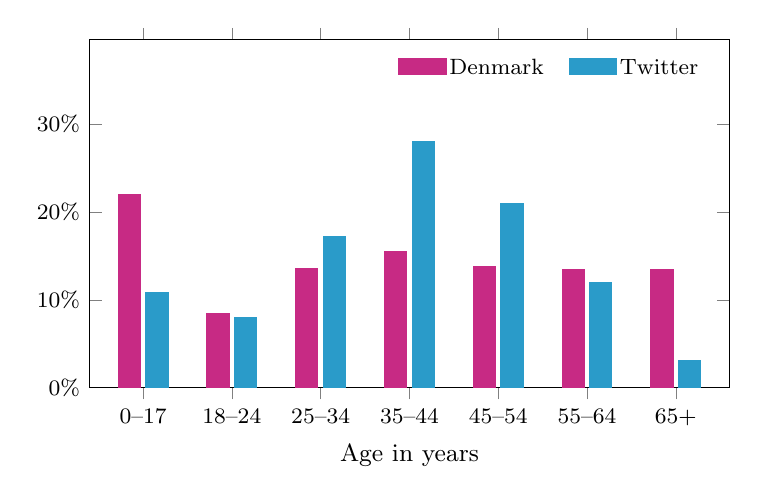
\begin{tikzpicture}
	\begin{axis}[
		small,
		ybar,
		area legend,
		enlargelimits=0.1,
		enlarge y limits=upper,	
		legend pos=north east,
		legend style={draw=none,legend columns=-1,cells={anchor=west},
		nodes={inner sep=1pt,below=-4pt},font=\footnotesize},
		legend style={/tikz/every even column/.append style={column sep=8pt}},
		xlabel={Age in years},
		symbolic x coords={0-17,18-24,25-34,35-44,45-54,55-64,65+},
		xtick=data,
		xticklabels={0--17,18--24,25--34,35--44,45--54,55--64,$65+$},
		xticklabel style={rotate=0,anchor=near xticklabel},
		yticklabel={$\pgfmathprintnumber{\tick}$\%},
		bar width=8pt,
		ymin=0,
		ymax=36,
		width=.8\textwidth,
		height=6cm
	]
	\addplot[magenta!80!black,fill=magenta!80!black] coordinates {
		(0-17,21.98)
		(18-24,8.39)
		(25-34,13.53)
		(35-44,15.48)
		(45-54,13.81)
		(55-64,13.40) 
		(65+,13.41)
	};
	\addplot[cyan!80!black,fill=cyan!80!black] coordinates {
		(0-17,10.82)
		(18-24,7.95)
		(25-34,17.22)
		(35-44,28.04)
		(45-54,20.97)
		(55-64,11.92) 
		(65+,3.09)
	};
	\legend{Denmark,Twitter}
	\end{axis}
\end{tikzpicture}
\end{center}
\vspace{-1em}
\caption{Age of Twitter Users and population of Denmark.}
\label{fig:population}
\end{figure}
\vspace{-1em}

Further details on this issue will not be concerned, but it is indeed necessary to correct collected data for sampling bias in order to draw any significant conclusions, such that the distribution of collected opinions indeed follows the target of the analysis.

Another more progressive approach for natural language data collection could be \emph{opinion seeking queries} as the one shown in (\ref{ex:OpinionQuery2}). Such queries are intended to ensure succinct reviews that clearly relate to the \emph{entity} in question (e.g.\ product or service) with respect to a specific \emph{topic of interest}.
\begin{numquote}
	What do you think about pricing at the Holiday Inn, London?
	\label{ex:OpinionQuery2}
\end{numquote}

This method might not seem that different from that of the previously mentioned Likert scales, but it still allows the reviewer to answer with a much broader sentiment and lets the reviewer argue for his/hers answer as shown in the examples (\ref{ex:OpinionAnswer}, \ref{ex:OpinionAnswer2}).
\begin{numquote}
	The price is moderate for the service and the location.
	\label{ex:OpinionAnswer}
\end{numquote}
\begin{numquote}
	Overall an above average hotel based on location and price   but not one for a romantic getaway!
	\label{ex:OpinionAnswer2}
\end{numquote}

\section{Sentiment of a text}
This section gives a succinct presentation of sentiment analysis, and introduce it as a research field. The research in sentiment analysis has only recently enjoyed high activity cf.\ \cite{webDataMining}, \cite{omsa}, which probably is due to a combination of the progress in machine learning research, the availability of huge data sets through the Internet, and finally the commercial applications that the field offers. \citeauthor{webDataMining} \shortcite[chap.~11]{webDataMining} identify three \emph{kinds} of sentiment analysis:
\begin{itemize}
	\item \emph{Sentiment classification} builds on text classification principles, to assign the text a \emph{sentiment polarity}, e.g.\ to classify the entire text as either positive or negative. This kind of analysis works on \emph{document level}, and thus no details are discovered about the entity of the opinions that are expressed by the text. The result is somewhat coarse, e.g.\ it  seems to be hard to classify (\ref{ex:multipleSentiments}) as \emph{either} positive or negative, since it contains multiple opinions.
	\vspace{1em}
	\begin{numquote}
		The buffet was expensive, but the view is amazing.
		\label{ex:multipleSentiments}
	\end{numquote}
	\item \emph{Feature-based sentiment analysis} works on \emph{sentence level} to discover opinions about entities present in the text. The analysis still assigns \emph{sentiment polarities}, but on an entity level, e.g.\ the text (\ref{ex:multipleSentiments}) may be analyzed to express a negative opinion about the \emph{buffet}, and a positive opinion about the \emph{view}.
	\item \emph{Comparative sentence and relation analysis} focus on opinions that describes similarities or differences of more than one entity, e.g.\ (\ref{ex:relativeSentiments}).
	\vspace{1em}
	\begin{numquote1}
		The rooms at Holiday Inn are cleaner than those at Swissôtel.		
		\label{ex:relativeSentiments}		
	\end{numquote1}	
\end{itemize}

The kind of analysis presented by this thesis is closest to the \emph{feature-based sentiment analysis}, however \citeauthor{webDataMining} \shortcite[chap.~11]{webDataMining} solely describes methods that uses \emph{machine learning approaches}, whereas this thesis focuses on a \emph{formal logical approach}. The difference between these approaches, and arguments for basing the solution on formal logic will be disclosed in the next section, and further details on the overall analytic approach is presented in Chapter~\ref{chap:sentimentAnalysis}.

Finally \citeauthor{webDataMining} \shortcite[chap.~11]{webDataMining} identify two \emph{ways} of expression opinion in texts, respectively \emph{explicit} and \emph{implicit} sentiments. An explicit sentiment is present when the sentence directly expresses an opinion about a subject, e.g.\ (\ref{ex:explicitSentiment}), whereas an implicit sentiment is present when the sentence implies an opinion, e.g.\ (\ref{ex:implicitSentiment}). Clearly sentences can contain a mix of explicit and implicit sentiments.
\begin{numquote}
	 The food for our event was delicious.
	\label{ex:explicitSentiment}
\end{numquote}
\begin{numquote}
	 When the food arrived it was the wrong order.
	\label{ex:implicitSentiment}
\end{numquote}

Most research focus on the explicit case, since identifying and evaluating implicit sentiment is an extremely difficult task which requires a high level of domain specific knowledge, e.g.\ in (\ref{ex:implicitSentiment}) where most people would regard it as negative if a restaurant served another dish then what they ordered. To emphasize this high domain dependency \citeauthor{omsa} \shortcite{omsa} considers the sentence (\ref{ex:implicitSentiment2}), which in the domain of \emph{book reviews} implies a positive sentiment, but the exact same sentence implies a negative sentiment in the domain of \emph{movie reviews}.
\begin{numquote}
	 Go read the book!
	\label{ex:implicitSentiment2}
\end{numquote}

The thesis will thus focus on the explicit case, since the implicit case was considered to simply require too much domain specific knowledge. This is due to two reasons, firstly the presented solution should be adaptable to \emph{any} domain, and thus tying it too closely to one type of domain knowledge was not an option, secondly the amount of domain knowledge required is in the vast number of cases simply not available, and thus needs to be constructed or collected. With that said the explicit case is neither domain independent, which is a problematic briefly touched in the next section, and detailed in Section~\ref{sec:semanticAnalysis}.

\section{The logical approach}
\label{sec:logicalApproach}
A coarse classification of the different approaches to sentiment analysis is to divide it into two classes: \emph{formal approaches} and \emph{machine learning approaches}. To avoid any confusion this thesis will present a method that belong to the formal class. 
\begin{itemize}
	\item \textit{Formal approaches} models the texts to analyze as a formal language, i.e.\ using a formal grammar. This allows a deep syntactic analysis of the texts, yielding the structures of the texts, e.g.\ sentences, phrases and words for \emph{phrase structure grammars}, and binary relations for \emph{dependency grammars}. Semantic information is then extractable by augmenting and inspecting these structures. The result of the semantic analysis is then subject to the actual sentiment analysis, by identifying positive and negative concepts, and how these modifies the subjects and objects in the sentences.

	\item \textit{Machine learning approaches} uses feature extraction to train probabilistic models from a set of labeled train data, e.g.\ a set of texts where each text is labeled as either positive or negative for the \emph{sentiment classification}-kind analysis. The model is then applied to the actual data set of which an analysis is desired. If the feature extracting \emph{really} does captures the features that are significant with respect to a text either being negative or positive, and the texts to analyze has the \emph{same} probability distribution as the training data, then the text will be classified correctly.
\end{itemize}

Notice that the presented classification only should be interpreted for the process of the actual sentiment analysis, not any preprocessing steps needed in order to apply the approach. Concretely the presented formal approach indeed do rely on machine learning techniques in order to efficiently identify lexical-syntactic properties of the text to analyze as will be covered in Chapter~\ref{chap:lexiconAcquisition}.

The motivation for focusing on the formal approach is two-folded: Firstly, different domains can have very different ways of expressing sentiment. What is considered as positive in one domain can be negative in another, and vice-verse. Likewise what is weighted as significant (i.e.\ either positive or negative) in one domain maybe completely nonsense in another, and again vice-verse, Scientific findings for this are shown by \citeauthor{domain}~\shortcite{domain}, but also really follows from basic intuition. Labeled train data are sparse, and since machine learning mostly assumes at least some portion of labeled target data are available this constitutes an issue with the pure machine learning approach. The end result is that the models follows different probability distributions, which complicates the approach, since such biases needs to be corrected, which is not a trivial task.

Secondly, machine learning will usually classify sentiment on document, sentence or simply on word level, but not on an entity level. This can have unintended results when trying to analyze sentences with coordination of sentiments for multiple entities, e.g.\ (\ref{ex:multipleSentiments}). The machine learning approaches that do try to analyze on entity level, e.g.\ \emph{feature-based sentiment analysis} by \citeauthor{webDataMining} \shortcite[chap.~11]{webDataMining}, relies on some fixed window for feature extraction, e.g.\ \citeauthor{webDataMining} \shortcite[chap.~11]{webDataMining} uses $n$-grams. As a result such methods fails to detect long distance dependencies between an entity and opinion stated about that entity. An illustration of this is shown by the potentially unbound number of \emph{relative clauses} allowed in English, e.g.\ (\ref{ex:longDistance}), where \emph{breakfast} is described as \emph{best}, however one would need to use a window size of at least $9$ to detect this relation, which is much larger then normally considered (\citeauthor{webDataMining} only considers up to trigrams).
\begin{numquote}
	The breakfast that was served Friday morning was the best I ever had!
	\label{ex:longDistance}
\end{numquote}

Formal logical systems are opposed to machine learning extremely precise in results. A conclusion (e.g.\ the sentiment value for a specific subject in a given text) is only possible if there exists a logical proof for this conclusion. 

\begin{quote}
\it\textbf{Thesis}: It is the thesis that a logical approach will be able to capture these complex and long distance relationships between entities and sentiments, thus achieving a more fine-grained entity level sentiment analysis.
\end{quote}

With that said, a logical approach indeed also suffers from obvious issues, most notable robustness, e.g.\ if there are missing, or incorrect axioms a formal logical system will not be able to conclude anything, whereas a machine learning approach will always be able to give an estimate, which might be a very uncertain estimate, but at least a result. This issue of robustness is crucial in the context of review texts, since such may not always be grammatical correct, or even be constituted by sentences. In Section~\ref{sec:realData} this issue will be addressed further, and throughout this thesis it will be a returning challenge. Details on the logical approach is presented in Chapter~\ref{chap:ccg}	

\section{Related work}
\label{sec:relatedWork}
In the following notable related work on sentiment analysis is briefly presented. As mentioned there are two main flavors of sentiment analysis, namely implicit and explicit. Most of the work found focus solely on the explicit kind of sentiment, just like this work does. 

Furthermore it seems that there is a strong imbalance between the \emph{formal approaches} and \emph{machine learning approaches}, with respect to amount of research, i.e.\ there exists a lot of research on sentiment analysis using machine leaning compared to research embracing formal methods. 

%\todo{Rewrite ...} This might not be that surprising, since wide-covering NLP becomes very ineffective (TODO: cite cite cite!) with pure formal methods. This thesis will thus also rely on machine learning methods for handling some of the initial NLP, however the actual sentiment analysis will be purely formal. 

Notably related work using formal approaches include \citeauthor{dependencySentiment} \shortcite{dependencySentiment}, who presents a method of extracting sentiment from dependency structures, and also focus on capturing long distance dependencies. As dependency structures simply can be seen as binary relations on words, it is indeed a formal approach. However what seems rather surprising is that in the end they only classify on sentence-level, and thus in this process loose entity of the dependency.

The most similar work on sentiment analysis found using a formal approach is the work by \citeauthor{valenceShifting} \shortcite{valenceShifting}. The paper presents a method to detect sentiment of newspaper headlines, in fact partially using the same grammar formalism that later will be presented and used in this work, however without the combinatorial logic approach. The paper focus on some specific problems arising with analyzing newspaper headlines, e.g.\ such as headline texts often do not constitute a complete sentence, etc. However the paper also present more general methods, including a method for building a highly covering map from words to polarities based on a small set of positive and negative seed words. This method has been adopted by this thesis, as it solves the assignment of polarity values on the lexical level quite elegantly, and is very loosely coupled to the domain. However their actual semantic analysis, which unfortunately is described somewhat shallow in the paper, seem to suffer from severe problems with respect to certain phrase structures, e.g.\ \emph{dependent clauses}.


\section{Using real data sets}
\label{sec:realData}

For the presented method to be truly convincing it is desired to present a fully functional \emph{proof of concept} implementation that shows at least the most essential capabilities. However, for such product to be demonstrated properly, real data is required. Testing in on some tiny pseudo data set constructed for the sole purpose of this demonstration would not be convincing. Chapter~\ref{chap:implementation} presents essential aspects of this \emph{proof of concept} implementation. 

An immediate concern that raises when dealing with real data sets is the possibility of incorrect grammar and spelling. A solution that would only work on \emph{perfect texts} (i.e.\ text with perfectly correct grammar and spelling) would not be adequate. %
Reasons for this could be that word is simply absent from the system's vocabulary (e.g.\ misspelled), or on a grammatical incorrect form (e.g.\ wrong person, gender, tense, case, etc.). 

Dealing with major grammatical errors, such as wrong word order is a much harder problem, since even small changes in, for instance, the relative order of subject, object, verb etc. may result in an major change in interpretation. Thus it is proposed, only to focus on minor grammatical errors such as incorrect form. Chapter~\ref{chap:evaluation} presents an evaluation of the implementation on actual review data.
